\section{Mask Attack}
\label{sec::chp5::mask-attack}

Mask attack is a method of guessing a password string when you have a partial representation of it, e.g. \password{p***w0r*}, or when individual characters are brute-forced using a chosen character set. Mask attack is a crucial password cracking technique as it allows us to make assumptions about the structure of the password, and therefore reduce the search space. Such assumptions about the structures are valid and practical. Moreover, it can aid in password recovery when the user has forgotten part of the password. Mask attacks can be used with the shoulder surfing attack, especially if the attacker has only captured small segments of the password. Despite the promising nature of it, the literature on this method is sparse. \hashcat provides a rich deterministic mask attack mode, and in the academic literature, a variant of this attack is described as \textit{Conditional Password Guessing (CPG)}~\cite{pasquini_improving_2021, xu_improving_2023}. We will refer to it as \textit{Mask Attack} because of its prominent use in practice, especially since \hashcat refers to it as mask attack. The aim is to correctly guess the missing characters (denoted by ``*'').

The purpose of this section is to review existing methods and to systemise the mask attack. The methods described in~\cite{pasquini_improving_2021, xu_improving_2023} follow a similar method; however, they have three drawbacks:
\begin{enumerate}
    \item Limited comparison to \hashcat and to the point that the mask attack method in \hashcat is ignored.
    
    \item Practicality of random masking of characters.
    
    \item A flow and model of the entire guessing process is not provided and thus it avoids the most crucial aspect of password guessing--speed and candidate generation.
\end{enumerate}

The brute-force method enumerates through masked characters in order to find a correct match. This method is predominantly used in practice using \hashcat.

% We can categorise the mask attacks into: 1) Probabilistic mask attack; 2) brute-force mask attack; 3) Dictionary + mask attack.
% 
% Mask attack scenarios can be conditioned on prior knowledge about the password. Knowledge about the structure, characters, language, knowledge about the user, and etc.

\subsection{Probabilistic Mask Attack}
\begin{figure}[ht]
    \centering
    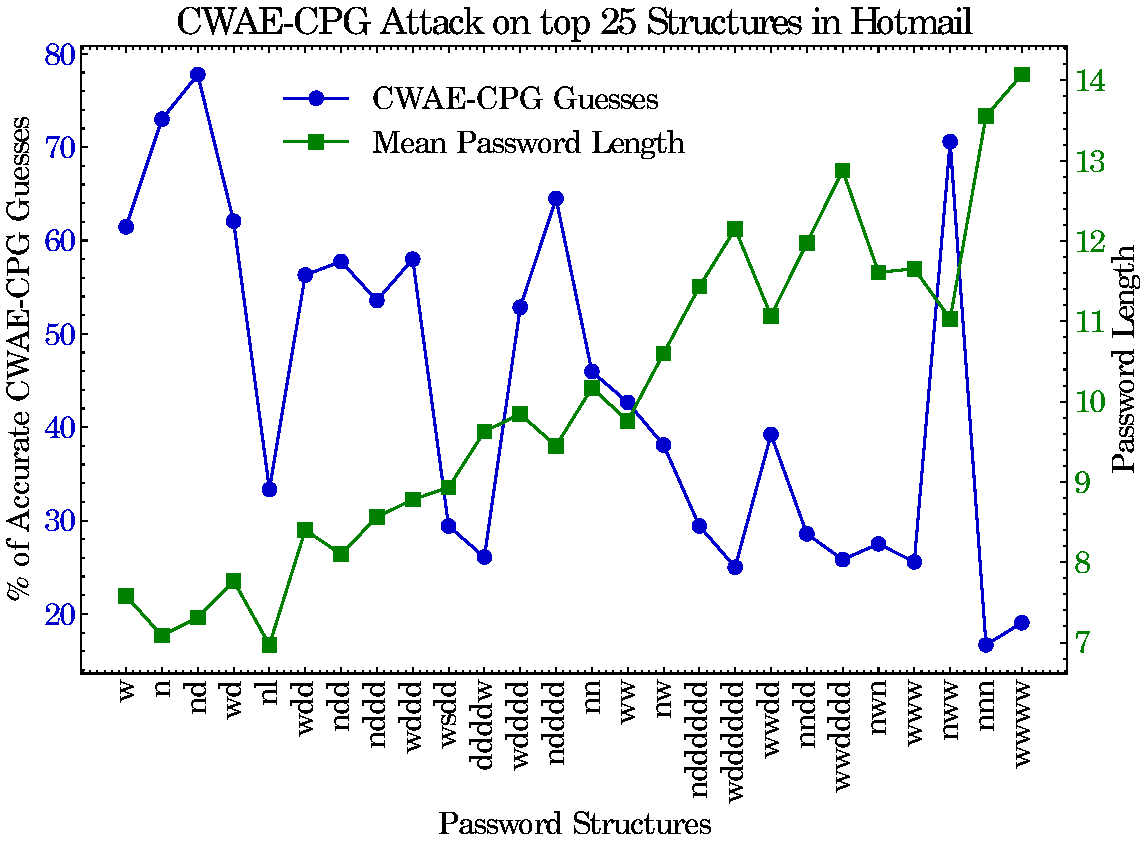
\includegraphics[scale=0.8]{figs/how_passwords/cwae_cpg_structures.pdf}
    \caption{Graph showing the percentage of guesses (left $y$-axis) with respect to the password structures in the \hmail dataset. Right $y$-axis shows the mean password length with respect to the password structures in the $x$-axis. \srcOwnFig}
    \label{fig::chp5::cwae_cpg_structures}
\end{figure}
\begin{figure}[ht]
\centering
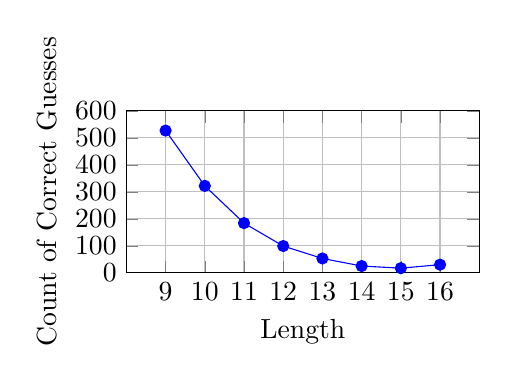
\begin{tikzpicture}
\begin{axis}[
    xlabel={Length},
    ylabel={Count of Correct Guesses},
    xmin=8, xmax=17,
    ymin=0, ymax=600,
    xtick={9,10,11,12,13,14,15,16},
    ytick={0,100,200,300,400,500,600},
    grid=major,
    width=0.5\textwidth,
    height=0.3\textwidth,
]
\addplot[color=blue, mark=*] coordinates {
    (9, 527)
    (10, 322)
    (11, 184)
    (12, 99)
    (13, 53)
    (14, 25)
    (15, 17)
    (16, 30)
};
\end{axis}
\end{tikzpicture}
\caption{Graph showing the performance of \cwaecpg against length of passwords. Using the \hmail dataset for analysis. We see a significant drop off as the length of passwords increase.}
\label{fig:mask_guess_count}
\end{figure}
\begin{table}[ht]
    \footnotesize
    \caption{Deep Learning and Probabilistic Masking Attacks literature.}
    \label{tab:my_label}
    \centering
    \begin{tabular}{ccccc}
        \toprule
        Exp & Train & Validation & Length & n \\
        \midrule
        CWAE-CPG \cite{pasquini_improving_2021} & Rockyou & Linkedin & $9 \leq L \leq 16$ & $10^7$ \\
        PassBERT \cite{xu_improving_2023} & Rockyou & NeoPets/Cit0day & $9 \leq L \leq ?$ & $10^7$ \\
        \bottomrule
    \end{tabular}
\end{table}
There are two notable models to be aware of at the time of writing: \cwaecpg uses a deep learning model based on the Wasserstein Auto-Encoder~\cite{tolstikhin_wasserstein_2019}. \passbert uses the BERT~\cite{devlin_bert_2019} architecture to model the password using the masking paradigm. These methods will often learn representation at word level, or structural patterns due to common passwords. These models condition the guess on some known characters in the password. The following shows the original password on the left and the \textit{template}\footnote{The reader may use the following website to try the masking algorithm on their own inputs: \url{https://sirvan3tr.github.io/tools/pwd/pwd_masker.html}} or masked password on the right.
\[
\text{\password{passw0rd123}} \rightarrow \text{\password{p***w0r*1*3}}
\]
The models then use deep learning techniques to learn to guess the masked characters or \textit{wild cards} (denoted by ``*''.)

We hypothesise that these methods will not do well against passphrases, or uncommon structures. For example, \password{TheTrooper} $\rightarrow$ \password{*h*****per} has too many masked characters to identify it as two words. Due to the 16 character limit as well, the model's outcome will be biased towards passphrases--which as we discussed are the strongest password structures.

We evaluated \cwaecpg\ against our labelled \hmail dataset to better understand the models performance against different password structures, the results are shown in Figure \ref{fig::chp5::cwae_cpg_structures}. For each password in the labelled \hmail dataset, we generated a template as per the \cwaecpg\ masking algorithm; then we evaluated each template (i.e. masked password) using the implementation and checkpoints released by the authors; finally for each password structure we calculated the percentage of passwords that were guessed correctly within $10^7$ guesses. Simpler structures (left side) tend to be shorter and more guessable; More complex structures (right side) tend to be longer and less guessable. Though the performance of \cwaecpgnocite\ seems correlated with the length of the password, we think the complexity is not necessarily the length but the fact that longer passwords in the dataset are composed using multiple words, dates, and names. This is further proof for NCSC's recommendation of composing these secrets using at least three random words.

Features of the training data, such as language, password structures, and date of breach, could effect the performance of the model. For example: Given a password dataset $D_t$ released at time $t$, we hypothesise that passwords containing temporal features (like years and dates) follow a time-dependent distribution $p_t(y)$ that heavily favours years closer to and preceding the release date $t$. This creates a fundamental challenge for password guessing models: when a model trained on an older dataset (e.g., $D_{2009}$) is evaluated on a newer dataset (e.g., $D_{2020}$), it encounters significant temporal distribution shift, as the training data lacks examples of passwords containing more recent years. For instance, while passwords like \password{password2018} might be common in $D_{2020}$, they would be entirely absent from $D_{2009}$, leading to poor generalization performance for passwords containing post-2009 temporal features.

%\subsection{Mask Attack Model}

\begin{figure}[t]
    \centering
    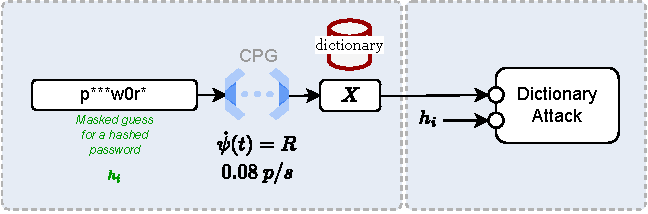
\includegraphics[scale=1.1]{figs/how_passwords/cpg.pdf}
    \caption{Data flow and model of a probabilistic mask attack or CPG. These methods thus far have randomly masked a password string and then generated a set of potential candidates. These candidates are then used to perform a dictionary attack. $\dot \psi(t)$ represents the rate of password generation. Note, an offline attack scenario is considered here.}
    \label{fig:masking-model}
\end{figure}
%The need for systematisation of mask attack is exemplified by the following. What \hashcat describes as a mask, e.g. \texttt{"?l?l?l?l?l"}, is described as a \textbf{template} in \cwaecpg and as a \textbf{pivot} in \passbert. Whilst we understand template, it is much harder to argue for the use of the term ``pivot''.
%
%A system conducting a probabilistic mask attack will use algorithms as follows.
%\begin{enumerate}[itemsep=0pt, parsep=0pt, leftmargin=12pt]
%    \item \textbf{\textsc{Mask}(1):} Let $x \in \mathcal{P}$, where $\mathcal{P}$ is the set of all possible passwords, $c_{min} \in \mathbb{N}$, and $m_{min} \in \mathbb{N}$. Define a masking function $f_1 : \mathcal{P} \times \mathbb{N} \times \mathbb{N} \rightarrow \mathcal{P}$ such that $f_1(x, c_{min}, m_{min}) = \hat{x}$, where $\hat{x}$ is the masked version of $x$, ensuring that at least $m_{min}$ characters are masked and at least $c_{min}$ characters remain unmasked.
%    
%    \item \textbf{\textsc{Mask}(2):} Given $x \in \mathcal{P}$ and $n \in \mathbb{N}$, define a masking function $f_2 : \mathcal{P} \times \mathbb{N} \rightarrow \mathcal{P}$ where $f_2(x, n) = \hat{x}$, and $\hat{x}$ is the result of masking $n$ distinct segments from the password $x$.
%    
%    \item \textbf{\textsc{Generate}(1):} Define a generation function $g_1 : \mathcal{P} \times \mathbb{N} \rightarrow 2^\mathcal{P}$, where $2^\mathcal{P}$ denotes the power set of $\mathcal{P}$, such that $g_1(\hat{x}, n) = X$, given a masked password $\hat{x}$, and $X$ is a set of $n$ potential password candidates.
%    
%    \item \textbf{\textsc{Generate}(2):} For a randomly masked password $\hat{x} \in \mathcal{P}$, define a generation function $g_2 : \mathcal{P} \rightarrow \mathcal{C}$, where $\mathcal{C}$ is the charset used to construct potential candidates, such that $g_2(\hat{x}) = y$. For example, $g_2(\text{"p***sw0rd"}) = \text{"p[l][l][l]sw0rd"}$, where $[l]$ indicates a placeholder for characters from a specified charset to be brute-forced.
%    
%    \item \textbf{\textsc{Filter}:} Define a filtering function $h : 2^\mathcal{P} \times \mathcal{P} \rightarrow 2^\mathcal{P}$, given a set of potential candidates $X \subseteq \mathcal{P}$ for masked password $x \in \mathcal{P}$, such that $h(X, x) = \hat{X}$, where $\hat{X} \subseteq X$ and $|\hat{X}| \ll |X|$. This function filters and significantly reduces the number of potential candidates by applying a set of predefined criteria or heuristics.
%\end{enumerate}

% The purpose of this section is to prove their unpracticality. The dangers of methods like this can feed into password composition policies and password complexity. The dangers are that we underestimate the real world and password guessing capabilities in the real world.

% PassBERT generates at 4.54 pwds/s, and CWAE-CPG at 0.08 pwds/s.


%   \begin{algorithm}
%     \footnotesize
%     \caption{Dynamic PCA}
%     \Comment{$\theta_{\mathrm{exp}}$ is globally given, and initially set to $\infty$.}
%     \Function{ExpandBasisIfInteresting($B$, $\Sigma$, $\vec{x}$)}{
%       \If{$\var{loss} > \theta_{\mathrm{exp}}$}{
%         $\var{loss} \assign \sqrt{\lVert \vec{x} \rVert^2 - \lVert \vec{x}^T B \rVert^2}$
%           \Comment{By Pythagoras}
%         $B, \Sigma \assign \FuncCall{Append}{$B$, $\Sigma$, $\vec{x}$}$\;
%         $B \assign \FuncCall{GramSchmidt}{$B$}$\;
%       }
%       $\theta_{\mathrm{exp}} \assign \FuncCall{UpdateLoss}{$\theta_{\mathrm{exp}}$, \var{loss}}$\;
%       \Return{$B$, $\Sigma$}\;
%     }
%     \Function{PeriodicDecompose($B$, $\Sigma$)}{
%       \If{\FuncCall{IsOneMinutePassed}{}}{
%         $B, \Sigma \assign \FuncCall{PCA}{$B$, $\Sigma$}$\;
%       }
%       \Return{$B$, $\Sigma$}\;
%     }
%     \Comment{The main function}
%     \Function{DynPCA($B$, $\Sigma$, $\vec{x}$, $s$)}{
%       $B, \Sigma \assign \FuncCall{ExpandBasisIfInteresting}{$B$, $\Sigma$, $\vec{x}$}$\;
%       $\Sigma \assign \FuncCall{UpdateCovMatrix}{$B$, $\Sigma$, $\vec{x}$, $s$}$\;
%       $B', \Sigma' \assign \FuncCall{PeriodicDecompose}{$B$, $\Sigma$}$\;
%       \Return{$B'$, $\Sigma'$}
%     }
%   \end{algorithm}

% \begin{algorithm}
% \footnotesize
% \DontPrintSemicolon
%   
%   \KwData{\\%
%   $\bm{s}$ Password string \\
%   $\bm{p}$ Probability, default=0.5 \\
%   $\bm{w}$ Minimum number of wildcards, default=5 \\
%   $\bm{c}$ Minimum number of normal characters, default=4}
%   \KwResult{A string with randomly replaced characters by wildcards '*' based on probability p, ensuring at least $w$ wildcards and $c$ characters remain unchanged.}
%   
%   \Function{CreateMask($s, p, w, c$)}{
%   %\SetKwProg{Fn}{Function}{:}{}
%   %\Fn{\FMain{password, p, w\_min, char\_min}}{
%         \If{$s.len < w + c$}{
%             \KwThrow{Password length must be at least the sum of $w$ and $c$.}
%         }
%         
%         \While{True}{
%         %\( x = \{c_1, c_2, \ldots, c_n\} \)
%         $x$ \assign s
% 
%             \For{$i = 0$ to $x.len$}{
%             $x[i] = 
%           \begin{cases} 
%            * & \text{if } \text{rand}() < p, \\
%            x[i] & \text{otherwise},
%           \end{cases}$
%             }
%             \If{$w$ $\leq$ count(* in x) $\leq s.len - c$}{
%                 \KwRet{x}
%             }
%         }
%   }
% \caption{Create a mask for the given password}
% \label{algo:probmask}
% \end{algorithm}

%Partial mask attacks, where a portion of the password is already fixed, has a significant advantage over other methods of attack. Therefore, the experiments and comparisons must reflect this.
%
%The method of masking also makes a significant difference. The methods in the literature \cite{pasquini_improving_2021, xu_improving_2023} are random masking with a probability of 0.5 as shown in Algorithm \ref{algo:probmask}. 
%
%Let us develop a practical model of an offline attack scenario given that CWAE-CPG also compared their method to other offline guessing techniques.
%
%Per our model, as seen in Figure \ref{fig:masking-model}, the secondary aim of a probabilistic masking attack is to reduce the search space from that of the deterministic masking attack (assuming we have the same mask). $|C| \ll S_d$

